\section{Observation and Calculation}
The appendix includes all the screenshots of the SEELab3 software used in the following sections.

\subsection{Transistor characteristics}
The following figure shows the obtained output characteristics of the given NPN transistor.
    \begin{figure}[h]
        \centering
        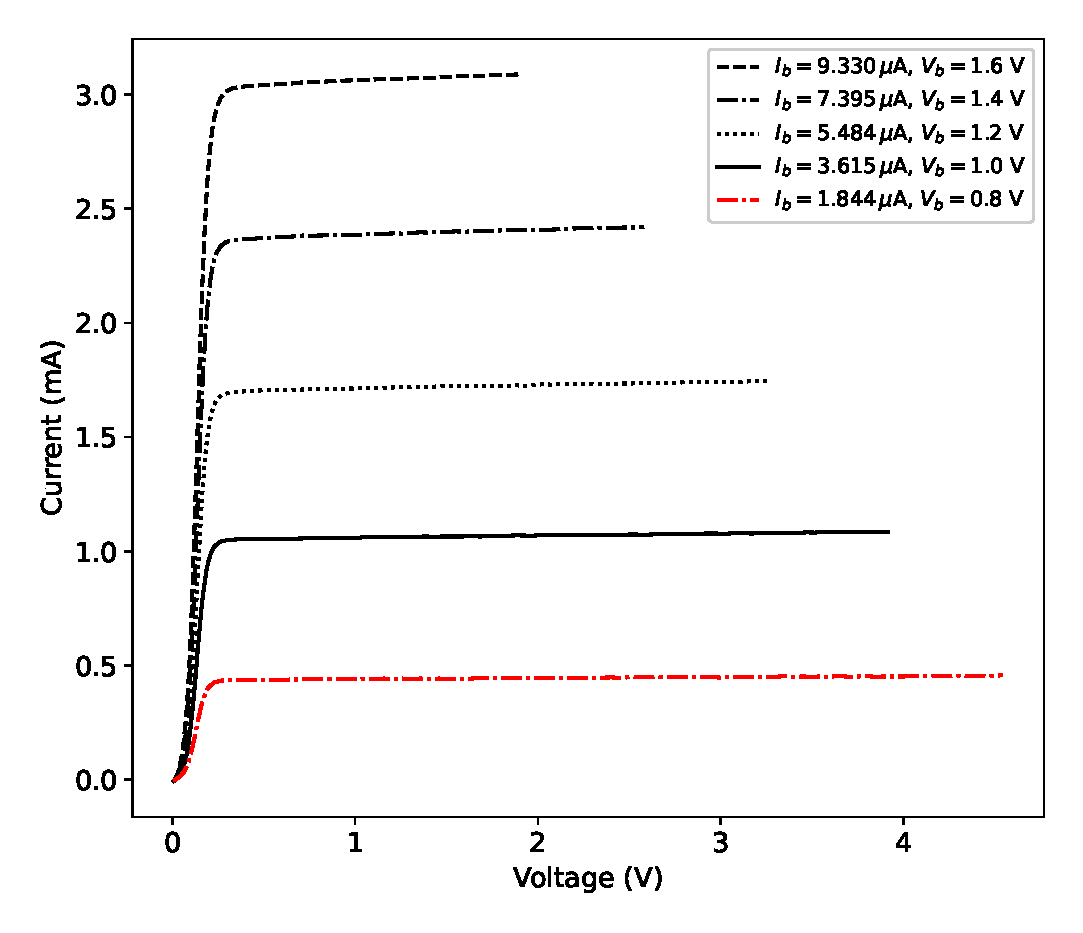
\includegraphics[width=1\columnwidth]{images/npn.eps}
        \caption{Current vs. Voltage Output characteristics of an NPN transistor in CE mode}
    \end{figure}

\subsection{Astable multivibrator with IC 555}

We have tested the astable multivibrator circuit for three different resistor combinations as give below.
\subsubsection{$f \approx 1.2$ kHz}
\begin{itemize}
    \item $R_A=10$ \kohm, $R_B=1$ \kohm
    \item $C_T=96.8$ nF
\end{itemize}

\begin{table}[H]
    \centering
    \begin{tabular}{|c|c|c|c|}\hline
        Parameter & Theoretical & Observed & Error \\ 
        & Value       & Value    &       \\ \hline 
        $f_\text{osc}$   & 1239.7 $\pm$ 0.6 Hz & 1230.4 Hz & $-0.3\%$  \\ \hline
        Duty Cycle       & 91.6 $\pm$ 0.02 \% & 91.7\%  & $-0.1\%$ \\ \hline
    \end{tabular}
\end{table}
\begin{figure}[H]
    \centering
    \includegraphics[width=0.9\columnwidth]{images/5551.eps}
    \caption{Voltage vs time graph for Astable multivibrator with parameters given above}
\end{figure}

\subsubsection{$f \approx 496$ Hz}
\begin{itemize}
    \item $R_A=10$ \kohm, $R_B=10$ \kohm
    \item $C_T=96.8$ nF
\end{itemize}

\begin{table}[H]
    \centering
    \begin{tabular}{|c|c|c|c|}\hline
        Parameter & Theoretical & Observed & Error \\ 
        & Value       & Value    &       \\ \hline 
        $f_\text{osc}$   & 495.9 $\pm$ 0.3 Hz & 487.2 Hz & $-0.1\%$  \\ \hline
        Duty Cycle       & 33.3 $\pm$ 0.01 \% & 31.8\%  & $-0.5\%$ \\ \hline
    \end{tabular}
\end{table}
\begin{figure}[H]
    \centering
    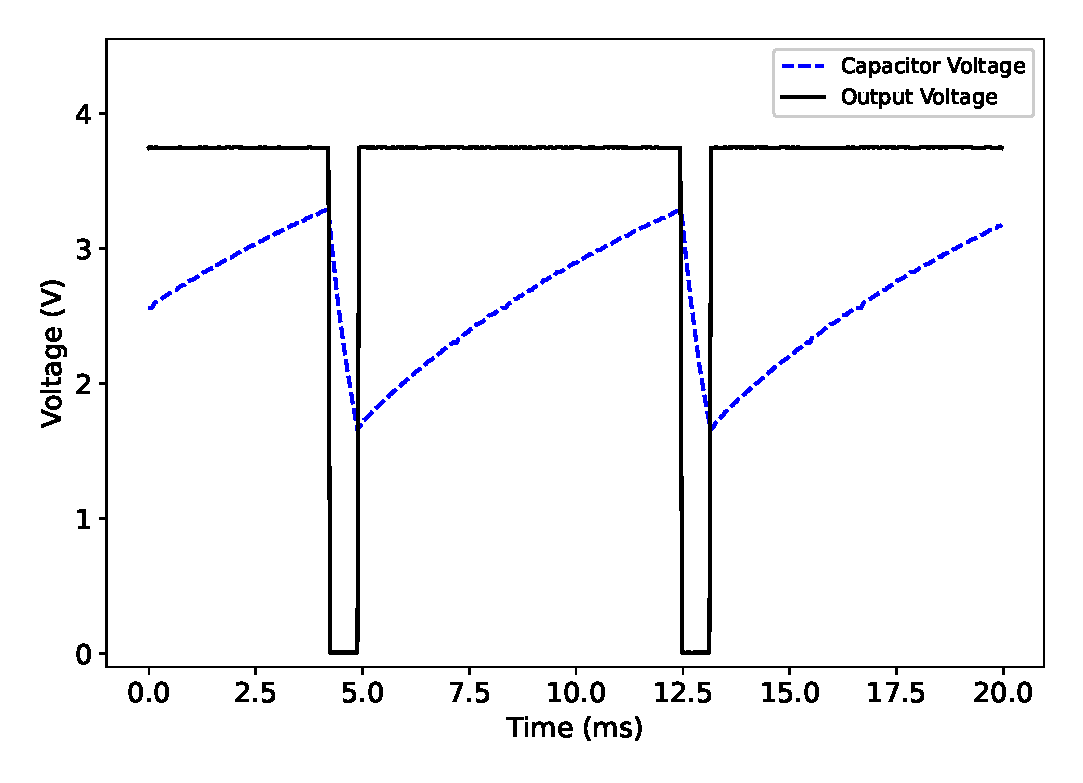
\includegraphics[width=0.9\columnwidth]{images/5552.eps}
    \caption{Voltage vs time graph for Astable multivibrator with parameters given above}
\end{figure}

\subsubsection{$f \approx 120$ Hz}
\begin{itemize}
    \item $R_A=100$ \kohm, $R_B=10$ \kohm
    \item $C_T=96.8$ nF
\end{itemize}

\begin{table}[H]
    \centering
    \begin{tabular}{|c|c|c|c|}\hline
        Parameter & Theoretical & Observed & Error \\ 
        & Value       & Value    &       \\ \hline 
        $f_\text{osc}$   & 123.9 $\pm$ 0.7 Hz & 119.7 Hz & $-0.2\%$  \\ \hline
        Duty Cycle       & 83.3 $\pm$ 0.05 \% & 91.7\%  & $-8.7\%$ \\ \hline
    \end{tabular}
\end{table}
\begin{figure}[H]
    \centering
    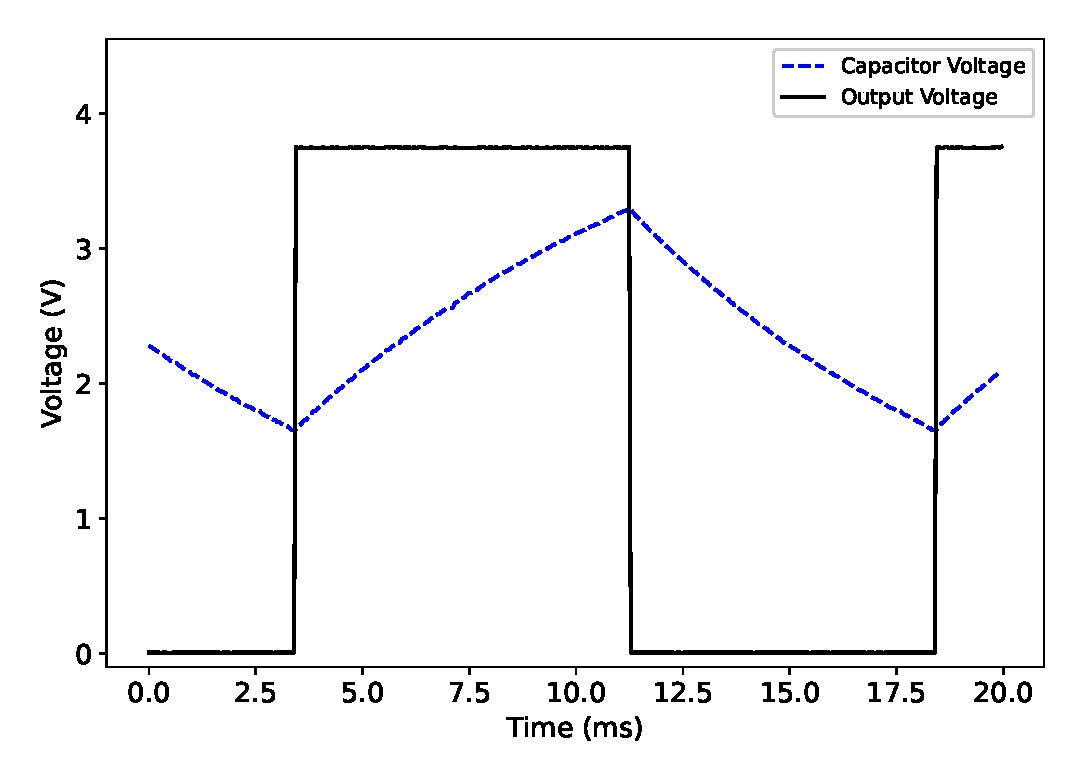
\includegraphics[width=1\columnwidth]{images/5553.eps}
    \caption{Voltage vs time graph for Astable multivibrator with parameters given above}
\end{figure}
    
\subsection{EM induction}
    
The emf vs. time graphs for the magnet dropped at two different heights while the coil was fixed just above the ground is shown below.
\begin{figure}[H]
    \centering
    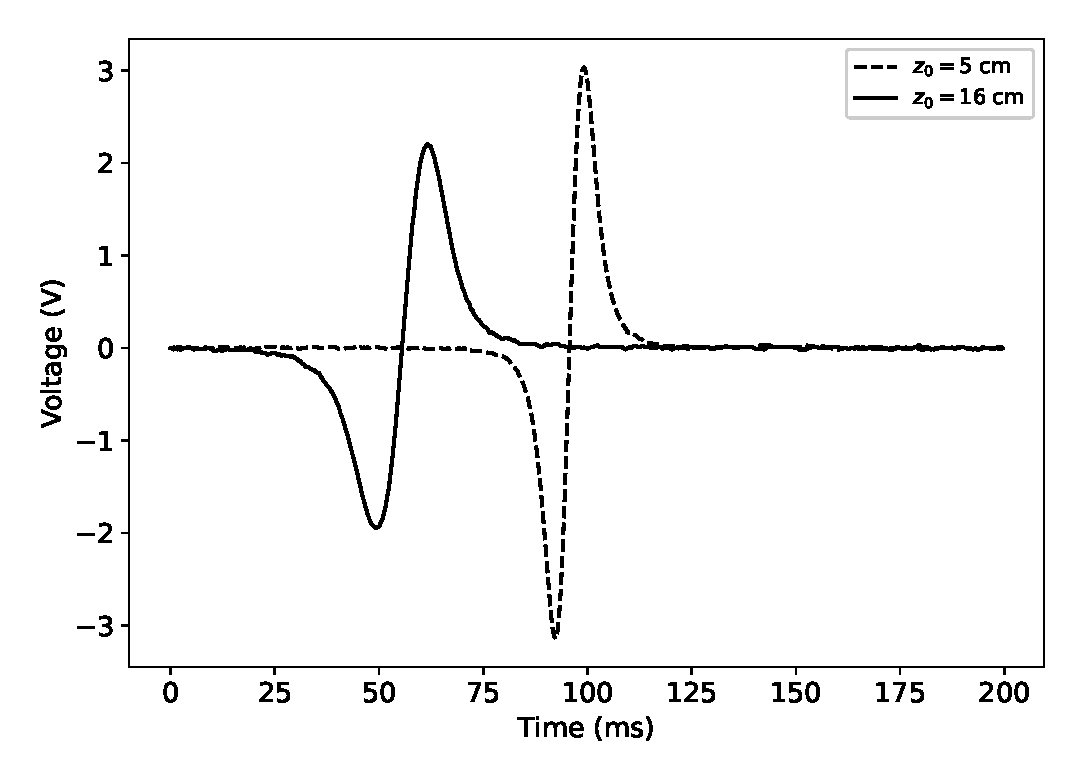
\includegraphics[width=1\columnwidth]{images/em.eps}
    \caption{Emf versus time graph for a vertically dropping magnet}
\end{figure}

From \hyperref[eq:4]{Equation 5} we have

We know that: $z_o=$ initial position of the magnet.
Also given:
$N=5000$,
$R = 0.002 m$
For both the cases,
\begin{itemize}
    \item $z_0 = 5$ cm, $t = 115$ ms, $emf = 3.139$ V
    This gives us $m = 7.61$ Am$^2$.
    \item $z_0 = 16$ cm, $t = 181$ ms, $emf = 2.208$ V
    This gives us $m = 9.97$ Am$^2$.
\end{itemize}

Thus, $m=8.79$ Am$^2$

\subsection{Determination of $g$ using Rod Pendulum}

The period of oscillation of the pendulum rod has been measured here with an accuracy of 100 $\mu$s. 

\begin{table}[H]
    \centering
    \begin{tabular}{|c|c|}\hline
    S.No. & Time (ms) \\ \hline
    0 & 520.280 \\
    1 & 520.545 \\
    2 & 520.199 \\
    3 & 520.390 \\
    4 & 519.956 \\
    5 & 520.428 \\
    6 & 519.872 \\
    7 & 520.264 \\
    8 & 519.822 \\
    9 & 520.096 \\
    10 & 519.858 \\\hline
    \end{tabular}
    \caption{Table of the period of oscillation of the pendulum rod measured as it passes by the phototransistor}
\end{table}

From this, the average value of $T_{avg} = 520.155$ ms. Plugging this is Eq. 6 (with $l=10$ cm),

\begin{align*}
    520.155 \times 10^{-3} &= 2\pi \sqrt{\frac{2\times 10 \times 10^{-2}}{3g}}\\
    \implies g &= 9.728 \text{ m/s}^2
\end{align*}

\subsection{Sound Beats}

Below is the visualisation of the sound beats produced by the combination of two sounds of frequency 3400 Hz and 3500 Hz respectively.

\begin{figure}
    \centering
    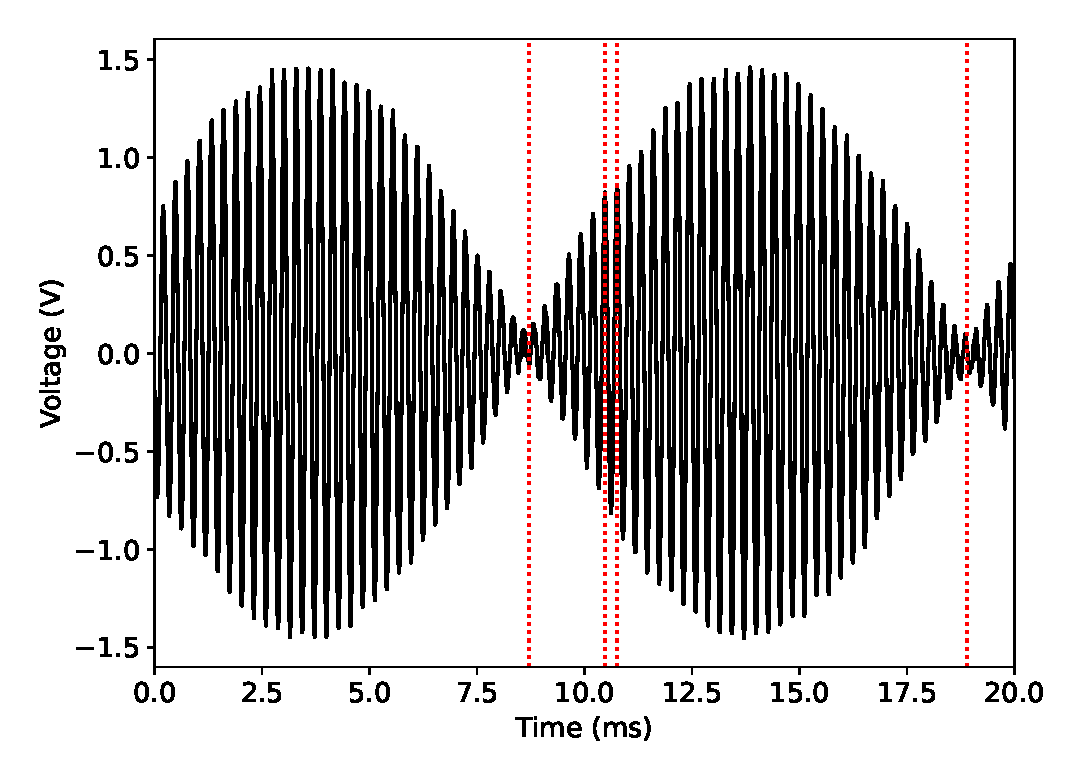
\includegraphics[width=1\columnwidth]{images/beat.eps}
    \caption{Voltage versus time graph observed b a microphone sensor.}
\end{figure}

Here, the time period of the small oscillations have been observed to be $T_1 = 0.29$ ms which equates to $f=3448.2$ Hz. Similarly, the time period of the envelope is observed to be roughly $T_2=10.2$ ms which equates to $f_b=98.1$ Hz. This is roughly equal to the theoretical value of $f=(f_1+f_2)/2=3450$ Hz and $f_b=(f_1-f_2)=100$ Hz.

\section{Error analysis}

\subsection{Astable Multivibrator}
In $IC 555$ multivibrator circuit the observed value of frequency and duty cycle is different from the theoretical value.

There may be several reasons for the high error in the observed values of frequency and duty cycle in the circuit using IC555. One possible reason is the difference between the actual values of resistors and capacitors used in the circuit and the ideal values assumed during calculations, which can affect the frequency and duty cycle. Another factor could be a loose connection or instability in the circuit, resulting in variations in the observed values.

The percentage errors in the calculated values have been mentioned in the previous section. The uncertainity in the theoretical values have been derived using the error propagation formula.

\subsection{EM Induction}
Similarly, the calculated magnetic moment may also have errors. Other forces such as air resistance and Lenz force, which are neglected in the calculations, could contribute to the error. Additionally, inaccuracies in the measured values of resistance (R) and distance (z) used in the calculations can also lead to errors in the magnetic moment value.

The uncertainity in the measurement of $m$ can be derived using the error propagation formula, using the uncertainity in $z_0$ which is 0.1 cm and the uncertainity in $V$ which is 0.001 V. $\Delta m$ comes out to be $0.05$ and $0.11$ for $z_0=5$ and 16 cm respectively.

\subsection{Determination of $g$ using Rod Pendulum}

The standard deviation of $T_{avg}$ from Table I is measured to be $\Delta T = 0.252$ ms. Hence by using error propagation, we can find the uncertainity in measurement of $g$ using 

\begin{align*}
    \frac{\Delta g}{g} &= \frac{2\Delta T}{T_{avg}}\\
    \implies \Delta g &= 9.728 \times \frac{0.252}{520.155}\\
    &= 0.005 \text{ m/s}^2
\end{align*}

where we assume $\Delta l = 0$. Hence, we have achieved remarkable precision in the measurement of $g$ here.


In summary, the high error in the observed values of frequency, duty cycle, and magnetic moment may be attributed to various factors, incluing differences in actual component values, circuit instability, neglected forces, and inaccuracies in measured values.